\documentclass[border=8pt]{standalone}
% Shared preamble for IronClaw thesis figures (standalone TikZ).
\renewcommand{\familydefault}{\sfdefault}
\usepackage{tikz}
\usetikzlibrary{arrows.meta,positioning,calc,fit,backgrounds,shapes.geometric,shapes.misc}

% IronClaw palette (matches slides.tex)
\definecolor{IronDark}{HTML}{1A2B3C}
\definecolor{IronBlue}{HTML}{2E86AB}
\definecolor{IronTeal}{HTML}{06A77D}
\definecolor{IronOrange}{HTML}{F18F01}
\definecolor{IronRed}{HTML}{C73E1D}
\definecolor{IronLight}{HTML}{F4F7F9}
\definecolor{IronGray}{HTML}{5D6D7E}

\tikzset{
  figtitle/.style={font=\large\bfseries\color{IronDark}, align=center},
  hostbox/.style={draw=IronBlue, rounded corners=5pt, fill=IronBlue!8,
                  line width=1pt, align=center, font=\small\color{white}},
  hostfill/.style={draw=IronBlue, rounded corners=4pt, fill=IronBlue,
                   line width=0.8pt, align=center, font=\small\color{white},
                   text width=3.1cm, minimum height=0.85cm},
  guestfill/.style={draw=IronOrange, rounded corners=4pt, fill=IronOrange!85,
                    line width=0.8pt, align=center, font=\small\color{white},
                    text width=3.1cm, minimum height=0.85cm},
  guestsoft/.style={draw=IronOrange, rounded corners=4pt, fill=IronOrange!25,
                    line width=0.8pt, align=center, font=\small\color{IronDark},
                    text width=3.1cm, minimum height=0.75cm},
  arrow/.style={-{Latex[length=2.6mm,width=2mm]}, line width=0.9pt, IronDark},
  biarrow/.style={{Latex[length=2.6mm,width=2mm]}-{Latex[length=2.6mm,width=2mm]},
                  line width=0.9pt, IronDark},
  note/.style={font=\footnotesize\color{IronGray}, align=center},
}

\begin{document}
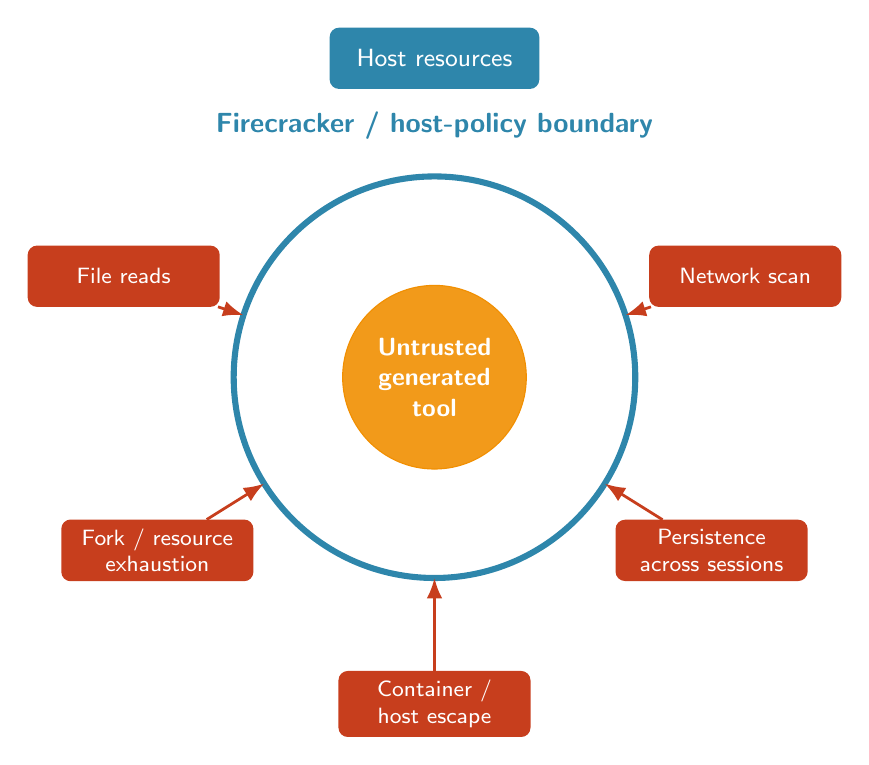
\begin{tikzpicture}
  \tikzset{
    attack/.style={draw=IronRed, fill=IronRed, text=white, rounded corners=3pt,
                   line width=0.8pt, align=center, font=\footnotesize,
                   text width=2.2cm, minimum height=0.75cm, inner sep=3pt},
    block/.style={-{Latex[length=2.6mm,width=2mm]}, line width=1pt, IronRed},
  }

  \def\ring{2.55}
  \def\rad{4.15}

  % boundary ring
  \draw[IronBlue, line width=2.2pt] (0,0) circle (\ring);

  % protected host + boundary label at top
  \node[draw=IronBlue, fill=IronBlue, text=white, rounded corners=3pt,
        line width=0.8pt, font=\small, minimum height=0.75cm, text width=2.4cm,
        align=center] at (0,4.05) {Host resources};
  \node[font=\normalsize\bfseries\color{IronBlue}] at (0,3.2)
        {Firecracker / host-policy boundary};

  % untrusted core
  \node[circle, draw=IronOrange, fill=IronOrange!90, text=white, align=center,
        font=\small\bfseries, text width=1.9cm, inner sep=2pt] at (0,0)
        {Untrusted generated tool};

  % attack vectors outside the boundary, arrows blocked at the ring
  \node[attack] (a1) at (162:\rad) {File reads};
  \node[attack] (a2) at (18:\rad)  {Network scan};
  \node[attack] (a3) at (212:\rad) {Fork / resource exhaustion};
  \node[attack] (a4) at (-32:\rad) {Persistence across sessions};
  \node[attack] (a5) at (270:\rad) {Container / host escape};

  \draw[block] (a1) -- (162:\ring);
  \draw[block] (a2) -- (18:\ring);
  \draw[block] (a3) -- (212:\ring);
  \draw[block] (a4) -- (-32:\ring);
  \draw[block] (a5) -- (270:\ring);

\end{tikzpicture}
\end{document}
